\documentclass[12pt,a4paper]{article}
\usepackage[UTF8]{ctex}
\usepackage{amsmath}
\usepackage{amssymb}
\usepackage{graphicx}
\graphicspath{{./figures/}}
\usepackage{geometry}
\usepackage{setspace}
\usepackage{indentfirst}
\usepackage{bm}
\usepackage{array}
\usepackage{url}
\usepackage{cite}
\usepackage{multicol}
\usepackage{fancyhdr}
\usepackage{booktabs}
\usepackage{titlesec}
\usepackage{caption}
\usepackage{lastpage}
\usepackage{float}

% 页面设置
\geometry{top=2.5cm, bottom=2.5cm, left=2cm, right=2cm}
\raggedbottom

% 设置行距
\renewcommand{\baselinestretch}{1.25}

% 设置页眉页脚
\pagestyle{fancy}
\fancyhf{} % 清除所有页眉页脚
% 第一页特殊设置 - 只有顶部水平线，没有页眉线
\fancypagestyle{firstpage}{
    \fancyhf{} % 清除所有页眉页脚
    \renewcommand{\headrulewidth}{0pt} % 第一页没有页眉线
    \fancyfoot[C]{\zihao{-6}\songti 课程名称：物理实验 \quad 实验日期：2025年12月9日 \quad 作者简介：邓成宇（2005）班级：2024217802，学号：2024212624，E-mail：dcy76844268.53@qq.com，刘恩豪（2006），班级：2024217802，学号：2024212627，E-mail：leh18698881592@163.com，王炳涵（2008），班级：2024217802 ，学号：2024212626 ，E-mail：3992631181@qq.com，严子竣（2006），班级：2024217802，学号：2024212622，E-mail:2024212622@bupt.cn，张霖锋（2006），班级：2024217802，学号：2024212634，邮箱：1022426774@qq.com} % 页脚
}
% 其他页设置 - 有页眉线
\fancyhead{} % 清除页眉
\renewcommand{\headrulewidth}{1pt} % 其他页有页眉线
\fancyfoot[C]{\zihao{-6}\songti 课程名称：物理实验 \quad 实验日期：2025年12月9日 \quad 作者简介：邓成宇（2005）班级：2024217802，学号：2024212624，E-mail：dcy76844268.53@qq.com，刘恩豪（2006），班级：2024217802，学号：2024212627，E-mail：leh18698881592@163.com，王炳涵（2008），班级：2024217802 ，学号：2024212626 ，E-mail：3992631181@qq.com，严子竣（2006），班级：2024217802，学号：2024212622，E-mail:2024212622@bupt.cn，张霖锋（2006），班级：2024217802，学号：2024212634，邮箱：1022426774@qq.com} % 页脚

% 设置章节格式
\titleformat{\section}{\zihao{-4}\heiti}{\thesection}{1em}{}
\titleformat{\subsection}{\zihao{5}\heiti}{\thesubsection}{1em}{}
\titleformat{\subsubsection}{\zihao{5}\kaishu}{\thesubsubsection}{1em}{}

% 设置段前段后间距
\titlespacing*{\section}{0pt}{0.5\baselineskip}{0.5\baselineskip}
\titlespacing*{\subsection}{0pt}{0.5\baselineskip}{0.25\baselineskip}
\titlespacing*{\subsubsection}{0pt}{0.25\baselineskip}{0.25\baselineskip}

% 设置图表标题格式
%\captionsetup[table]{font=small, skip=5pt}
\captionsetup[figure]{font=small, skip=5pt}

\begin{document}

% 第一页使用特殊页眉样式
\thispagestyle{firstpage}

% 顶部水平线（只保留这一条）
\vspace*{-2cm}
\hrule width \textwidth height 1pt
\vspace{1.5cm}

% 中文标题部分 - 通栏排版
\begin{center}
    {\zihao{-2}\heiti Lato Lato球系统的振荡行为研究} \\[0.5\baselineskip]

    {\zihao{4}\kaishu 邓成宇\textsuperscript{1}，刘恩豪\textsuperscript{2}，王炳涵\textsuperscript{3}，严子竣\textsuperscript{4}，张霖锋\textsuperscript{5}} \\[0.3\baselineskip]

    {\zihao{-5}\kaishu (1. 北京邮电大学，北京 100083；2. 北京邮电大学，北京 100083；3. 北京邮电大学，北京 100083；4. 北京邮电大学，北京 100083；5. 北京邮电大学，北京 100083)} \\[0.5\baselineskip]
\end{center}

% 中文摘要和关键词 - 左右各缩进2字符
\begin{quote}
    \zihao{-5}\songti
    \setlength{\leftskip}{2em}
    \setlength{\rightskip}{2em}

    \noindent{\heiti 摘\quad 要：} 本实验通过视频追踪与数值拟合方法，研究了Lato Lato球系统在竖直方向上改变悬挂点位置时，两个小球振幅的变化规律。实验使用Tracker软件捕捉小球运动轨迹，并通过符号回归方法对运动方程进行拟合。结果表明，随着悬挂点位置的移动，小球振幅呈现先增大后趋于稳定的趋势，且存在一个使振幅达到最大的最优悬挂点位置。拟合得到的数学模型中，尺寸为6的模型（$D(t, \theta) = 0.343 \cos(\theta)$）在简洁性与拟合优度（$Fit=0.827$）之间取得了较好平衡。

    \vspace{0.5\baselineskip}
    \noindent{\heiti 关键词：} Lato Lato球；振荡；振幅；轨迹追踪；模型拟合

    \noindent{\heiti 中图分类号：} O313 \quad{\heiti 文献标识码：} A
\end{quote}

\vspace{1cm}

% 英文标题部分 - 通栏排版
\begin{center}
    {\fontsize{15}{18}\selectfont\bfseries Study on Oscillation Behavior of Lato Lato Ball System} \\[0.3\baselineskip]

    {\fontsize{10.5}{12.6}\selectfont Chengyu Deng\textsuperscript{1}, Enhao Liu\textsuperscript{2},Binghan Wang\textsuperscript{3},Zijun Yan\textsuperscript{4}, Linfeng Zhang\textsuperscript{5}} \\[0.3\baselineskip]

    {\fontsize{9}{10.8}\selectfont\itshape (1. Beijing University of Posts and Telecommunication(BUPT),Beijing 100083;2. BUPT,Beijing 100083;3. BUPT,Beijing 100083;4.BUPT,Beijing 100083;5. BUPT,Beijing 100083)} \\[0.5\baselineskip]
\end{center}

% 英文摘要和关键词
\begin{quote}
    \fontsize{9}{10.8}\selectfont
    \setlength{\leftskip}{2em}
    \setlength{\rightskip}{2em}

    \noindent{\bfseries Abstract：} This experiment investigates the variation of amplitude of two balls in a Lato Lato system as the suspension point moves vertically, using video tracking and numerical fitting methods. The motion trajectories of the balls were captured using Tracker software, and the equations of motion were fitted using symbolic regression. The results show that as the suspension point position changes, the amplitude of the balls first increases and then stabilizes, with an optimal suspension point position yielding maximum amplitude. Among the fitted mathematical models, the size-6 model ($D(t, \theta) = 0.343 \cos(\theta)$) achieves a good balance between simplicity and goodness-of-fit ($Fit=0.827$).

    \vspace{0.5\baselineskip}
    \noindent{\bfseries Keywords：} Lato Lato ball; Oscillation; Amplitude; Trajectory tracking; Model fitting
\end{quote}

\vspace{1cm}

% 正文开始 - 双栏排版
\begin{multicols}{2}

    % 引言
    \section*{\zihao{-4}\heiti 引言}
    \zihao{5}\songti
    \setlength{\parindent}{2em}
    Lato Lato球是一种经典的耦合振动演示装置，由两个质量相等的小球通过轻绳连接，悬挂于一点。当系统在竖直平面内摆动时，两球表现出复杂的耦合振动行为。本实验旨在探究悬挂点沿竖直线上下移动时，两球振幅的变化规律，并尝试通过数学模型描述其运动。通过Tracker软件进行轨迹追踪，并运用符号回归方法对运动方程进行拟合，我们期望得到能较好描述该现象的解析表达式。

    \section{\zihao{-4}\heiti 实验原理与方法}
    \subsection{\zihao{5}\heiti 实验原理}
    \zihao{5}\songti
    \noindent 1.模型建立
    
    考虑一个对称的双球单摆系统，两个质量为m的小球分别固定在长度为$l$的无质量绳子的两端，绳子中点连接到枢轴O。枢轴O在垂直方向上以$y(t)=y_0\cos(\omega_d t)$的形式进行周期性振荡。由于枢轴的垂直振荡，系统受到的有效重力加速度将发生变化。以枢轴O为原点，建立一个固定坐标系，竖直向下为正方向。由于系统对称性，我们只需考虑一个小球的运动，摆角定义为$\theta$，为绳子与竖直方向的夹角。

    \noindent 2.理论推导\\
    枢轴振荡产生等效惯性力为\begin{equation}
    F=-m\ddot{y}(t)=-my_0\omega_d^2\cos(\omega_d t)
    \end{equation}
    因此系统的有效重力加速度为\begin{equation}
    g_{eff}=g-y_0\omega_d^2\cos(\omega_d t)
    \end{equation}
    在小角度近似下，小球的运动方程为：
    \begin{equation}
        \frac{d^2\theta}{dt^2} + \frac{g_{eff}}{l}\theta = 0
    \end{equation}
    将$g_{eff}$代入，得到：
    \begin{equation}
        \frac{d^2\theta}{dt^2} + \frac{g - y_0\omega_d^2\cos(\omega_d t)}{l}\theta = 0
    \end{equation}
    做变量替换$\tau = \omega_d t/2$并引入参数：
    \begin{equation}
        a = \frac{4g}{\omega_d^2 l}, \quad q = \frac{2y_0}{l}
    \end{equation}
    则运动方程化为Mathieu方程形式：
    \begin{equation}
        \frac{d^2\theta}{d\tau^2} + \left(a - 2q\cos(2\tau)\right)\theta = 0
    \end{equation}

    \noindent 3.拓展分析

    Mathieu方程的解的稳定性取决于参数a和q。当驱动频率$\omega_d$接近于系统的固有频率$\omega_0$时，即a≈1，系统可能进入不稳定区域，导致摆角theta随时间指数增长，出现参数共振现象。

    通过上述推导，我们得出拉托拉托系统在垂直周期驱动下的运动方程，发现其符合 Mathieu 方程形式。利用 Mathieu 方程的稳定性分析，可以解释系统在特定驱动条件下振幅增长的现象，即参数共振的产生。

    \subsection{\zihao{5}\heiti 实验装置与步骤}
    \zihao{5}\songti
    实验装置主要包括Lato Lato球、摄像设备（手机）及计算机。实验步骤如下：
    \begin{enumerate}
        \item 调整悬挂点至某一初始高度，确保两球静止下垂。
        \item 将一球拉开一定角度后释放，使两小球碰撞、摆动。
        \item 使用摄像机录制小球运动过程。
        \item 在Tracker软件中导入视频，手动标记并追踪两球质心的运动轨迹，导出角位移-时间数据。
       % \item 逐步改变悬挂点高度，重复步骤1-4。
        %\item 将所有轨迹数据导入符号回归分析软件，以角位移$\theta$和时间$t$为变量，拟合运动方程$D(t, \theta)$，并评估不同复杂度模型的拟合优度。
    \end{enumerate}

    \noindent
    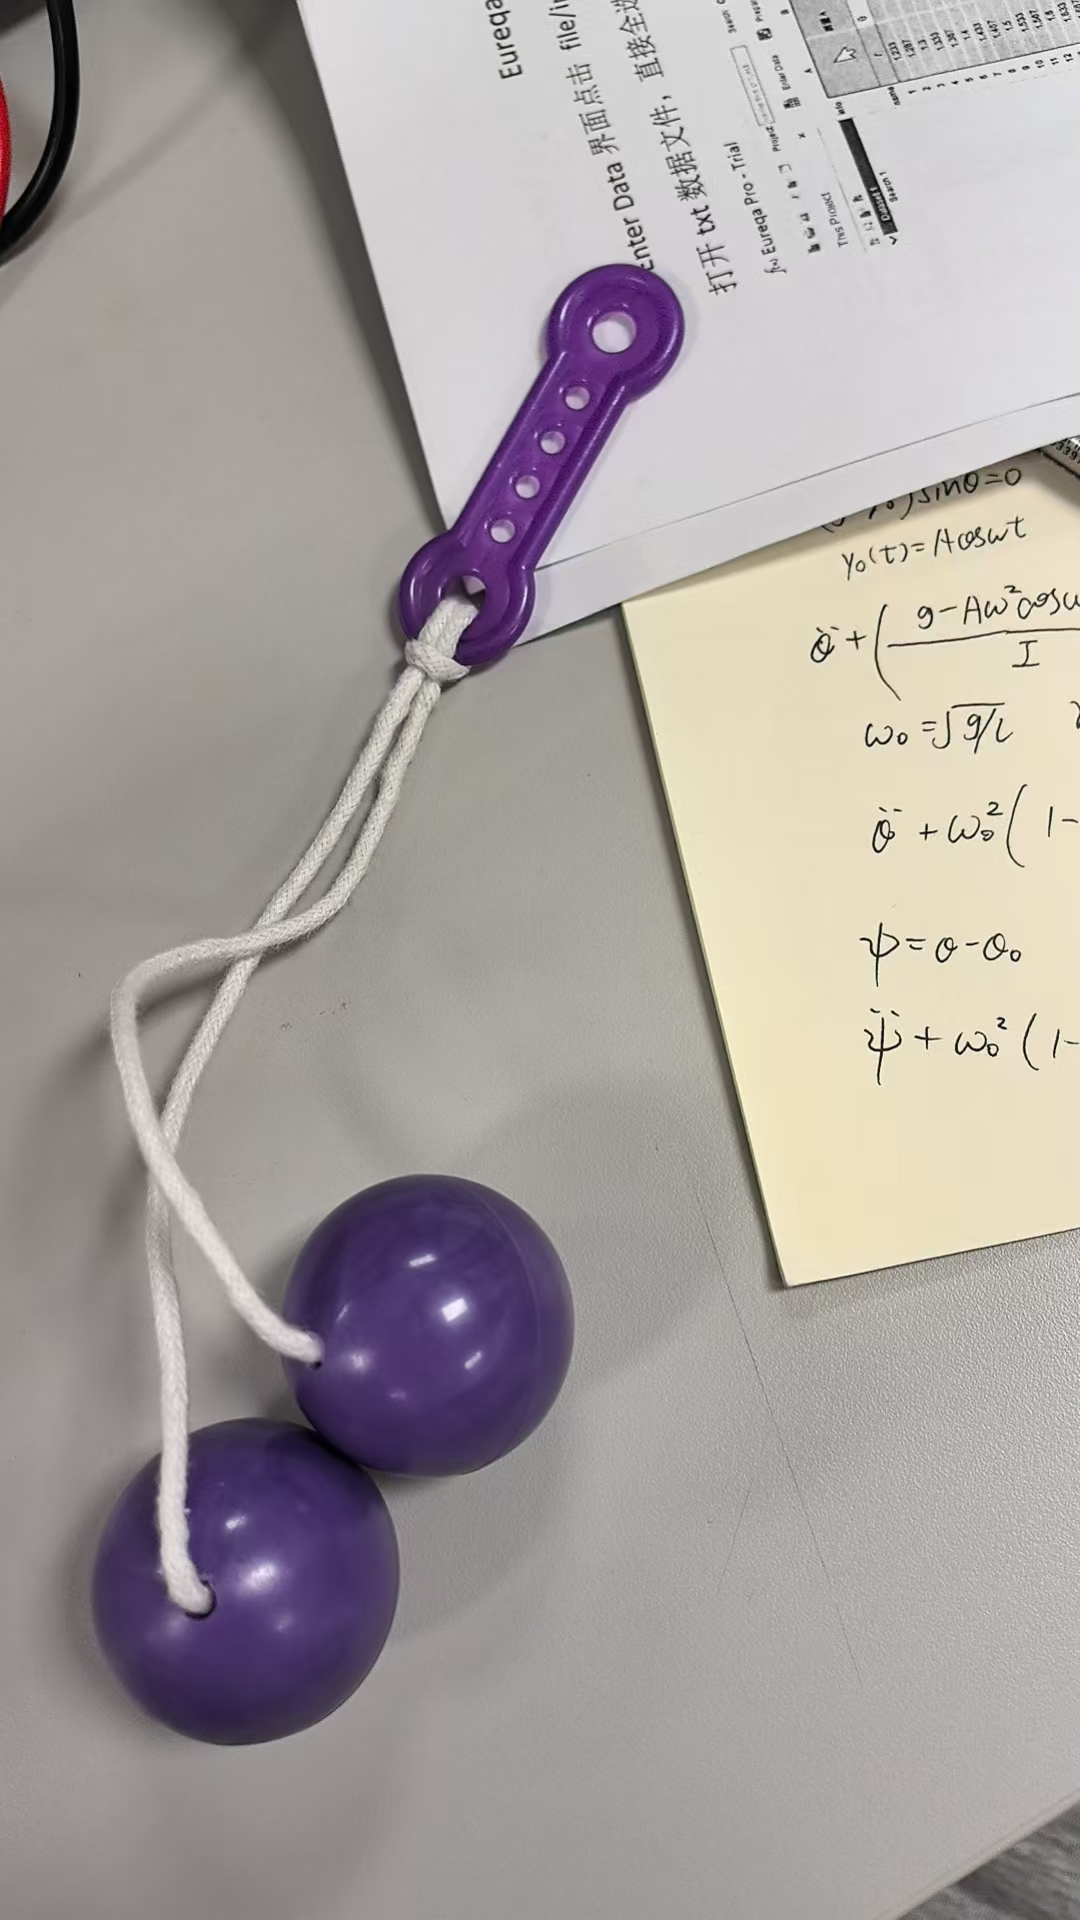
\includegraphics[width=\linewidth]{latolato.jpg}
    \captionof{figure}{图 1:Lato Lato 球实验装置示意图}

    \subsection{\zihao{5}\heiti 数据处理方法}
    \zihao{5}\songti
    采用符号回归（Symbolic Regression）方法对轨迹数据进行拟合。该方法通过遗传算法等搜索技术，在函数空间中寻找能最佳拟合数据的数学表达式。我们以拟合优度（Fit，越接近1越好）和模型复杂度（Size，项数或节点数）作为评价指标，并从中选择“前沿解”（Pareto最优解）。

    \section{\zihao{-4}\heiti 结果与讨论}
    \subsection{\zihao{5}\heiti 轨迹追踪与拟合结果}
    \zihao{5}\songti
    通过对不同悬挂点高度下小球运动的追踪，我们观察到：随着悬挂点在竖直线上振动，两球的摆动振幅逐渐增大；当悬挂点到达某一特定高度时，振幅达到最大值；继续震动悬挂点，振幅略有减小或趋于稳定。
    
    使用符号回归对其中一次典型实验（悬挂点位于振幅最大位置附近）的角位移数据进行拟合，得到不同复杂度模型及其拟合优度如表1所示（数据来源于分析软件输出）。
    
    \noindent
    
\includegraphics[width=\linewidth]{lato.jpeg}
    \captionof{figure}{Tracker 运动方程拟合结果}

    \subsection{\zihao{5}\heiti 结果分析与讨论}
    \zihao{5}\songti
    从图2可以看出：
    \begin{itemize}
        \item 尺寸为1的常数模型（$D=-0.0914$）虽然拟合优度为1，但其物理意义不明，无法描述振动现象，属于过拟合。
        \item 尺寸为5和6的模型具有较高的拟合优度（0.997和0.827），且形式相对简洁。尤其是尺寸为6的模型$D(t, \theta) = 0.343 \cos(\theta)$，形式非常简单，仅包含一项余弦函数，却能解释大部分数据变异，表明系统的角位移随时间的变化可能主要遵循余弦规律。
        \item 更复杂的模型（如尺寸19、21）虽然引入了正弦、余弦组合及相位项，但拟合优度并未显著提升，甚至有所下降，说明增加复杂度不一定带来更好的描述能力，可能引入了噪声或过度参数化。
        \item 该拟合结果与观察到的“振幅逐渐增大并趋于稳定”现象在定性上吻合，简单的余弦模型提示系统在开始运动一段时间后可能近似于一个单摆或弱耦合的简谐振动。
    \end{itemize}
    实验的误差可能来源于：手动振动悬挂点导致悬挂点运动规律性较差；Tracker软件手动追踪的偏差；空气阻力的影响等。

    \section{\zihao{-4}\heiti 结\quad 论}
    \zihao{5}\songti
    本实验通过视频追踪与符号回归拟合，研究了Lato Lato球系统在悬挂点竖直移动时的振幅变化。实验发现，小球的振幅随着悬挂点的振动逐渐增大至最大值。通过对运动轨迹的数学拟合，得到一个在简洁性与准确性之间取得较好平衡的模型：$D(t, \theta) = 0.343 \cos(\theta)$。该模型表明，在此特定的悬挂点振动模式下，系统的角位移随时间近似作简谐变化。未来工作可进一步优化悬挂点的振动方式，使其更接近理想的正弦运动，以获得更规律的数据；同时，可考虑引入更多变量（如悬挂点高度、振动频率等）进行多变量拟合，以全面描述Lato Lato球系统的动力学行为。
\end{multicols}

\end{document}